% note-setup-borderless.tex
% fenglielie@qq.com 2025-07-10

\documentclass{article}
\usepackage{amsmath,amsthm,amsfonts,amssymb}
\usepackage{mathtools}
\usepackage{mathrsfs}
\usepackage{bm}
\usepackage{extarrows}
\usepackage[a4paper, margin=1in]{geometry}
\usepackage{float}
\usepackage{indentfirst}
\usepackage{anyfontsize}
\usepackage{booktabs,multirow,multicol}
\usepackage[shortlabels,inline]{enumitem}
\usepackage{appendix}

\usepackage[dvipsnames]{xcolor}
\usepackage{graphicx}
\graphicspath{
    {./figure/}{./figures/}{./image/}{./images/}{./graphic/}{./graphics/}{./picture/}{./pictures/}
}
\usepackage{subcaption}

\usepackage[ruled,linesnumbered,noline]{algorithm2e}
\usepackage{listings}
\lstdefinestyle{simpleStyle}{
    basicstyle=\ttfamily\small,
    breaklines=true,
    keywordstyle=\color{blue},
    identifierstyle=\color{black},
    stringstyle=\color{violet},
    commentstyle=\color[RGB]{34,139,34},
    showstringspaces=false,
    numbers=left,
    numbersep=2em,
    numberstyle=\footnotesize,
    frame=single,
    framesep=1em,
}
\lstset{style=simpleStyle}

\usepackage[colorlinks=true,linkcolor=,urlcolor=magenta,citecolor=violet]{hyperref}

\renewcommand*{\proofname}{\normalfont\bfseries Proof}

\usepackage{thmtools}
\usepackage{tikz}
\usepackage{tikz-3dplot}

%% define environments

\declaretheorem[style=plain, name=Theorem, numbered=yes, numberwithin=section]{theorem}
\declaretheorem[style=plain, name=Theorem, numbered=no]{theorem*}

\declaretheorem[style=plain, name=Proposition, numbered=yes, sibling=theorem]{proposition}
\declaretheorem[style=plain, name=Proposition, numbered=no]{proposition*}

\declaretheorem[style=plain, name=Corollary, numbered=yes, sibling=theorem]{corollary}
\declaretheorem[style=plain, name=Corollary, numbered=no]{corollary*}

\declaretheorem[style=plain, name=Lemma, numbered=yes, sibling=theorem]{lemma}
\declaretheorem[style=plain, name=Lemma, numbered=no]{lemma*}

\declaretheorem[style=plain, name=Claim, numbered=yes, sibling=theorem]{claim}
\declaretheorem[style=plain, name=Claim, numbered=no]{claim*}

\declaretheorem[style=definition, name=Definition, numbered=yes, numberwithin=section]{definition}
\declaretheorem[style=definition, name=Definition, numbered=no]{definition*}

\declaretheorem[style=definition, name=Example, numbered=yes, numberwithin=section]{example}
\declaretheorem[style=definition, name=Example, numbered=no]{example*}

\declaretheorem[style=definition, name=Problem, numbered=yes, numberwithin=section]{problem}
\declaretheorem[style=definition, name=Problem, numbered=no]{problem*}

\declaretheorem[style=remark, name=Remark, numbered=yes, numberwithin=section]{remark}
\declaretheorem[style=remark, name=Remark, numbered=no]{remark*}

\declaretheorem[style=remark, name=Note, numbered=yes, numberwithin=section]{note}
\declaretheorem[style=remark, name=Note, numbered=no]{note*}

\declaretheoremstyle[headfont=\bfseries, bodyfont=\normalfont, spaceabove=3pt, spacebelow=3pt, qed=\ensuremath{\square}]{solutionstyle}

\declaretheorem[style=solutionstyle, name=Solution, numbered=yes, numberwithin=section]{solution}
\declaretheorem[style=solutionstyle, name=Solution, numbered=no]{solution*}

\usepackage[most]{tcolorbox}

\newcommand{\newtcbenvironment}[2]{
    \tcolorboxenvironment{#1}{#2, enhanced, breakable, sharp corners, boxrule=0pt, colframe=white}
    \tcolorboxenvironment{#1*}{#2, enhanced, breakable, rounded corners, boxrule=0pt, colframe=white}
}

%% define styles

\newtcbenvironment{theorem}{colframe=RoyalPurple, colback=RoyalPurple!8}
\newtcbenvironment{proposition}{colframe=RoyalPurple, colback=RoyalPurple!8}
\newtcbenvironment{corollary}{colframe=NavyBlue, colback=SkyBlue!8}
\newtcbenvironment{lemma}{colframe=NavyBlue, colback=SkyBlue!8}
\newtcbenvironment{claim}{colframe=NavyBlue, colback=SkyBlue!8}

\newtcbenvironment{definition}{colframe=ForestGreen, colback=ForestGreen!5}
\newtcbenvironment{example}{colframe=RawSienna, colback=RawSienna!5}
\newtcbenvironment{problem}{colframe=WildStrawberry!30, colback=WildStrawberry!5}

\newtheorem{exercise}{Exercise}

%define short cut notation
\newcommand{\g}{\mathfrak{g}}
\newcommand{\h}{\mathfrak{h}}

\title{Riemann Surfaces}
\author{Zihan Ke}

\begin{document}
\maketitle
\section*{Introduction}
Riemann Surfaces is the one-dimensional complex manifold. Also, it can be described as the one-dimensional complex algeraic curves. I first encounter the concept of Riemann Surfaces in complex analysis.Later I found that Riemann Surfaces is not only an interesting object to learn itself. Since it cna be described as algebraic curves, it also provides a path to the study of algebraic geometry. I want to learn algebraic geometry and Riemann Surfaces is a good place to start. 
OUr goal in this note is to obtain Riemann-Roch theorem and its application.
\newpage
\tableofcontents 
\newpage

\section{Riemann Surfaces and complex \textbf{manifolds}.}
\subsection{Holomorphic functions in 1-variable}
\subsection{Holomorphic functions in $n$-variables}
\subsection{Complex manifolds \& Riemann Surfaces.}

\begin{definition}
    Let $X$ be a \textbf{topological} space.
    \begin{enumerate}
        \item A $n$-dim \textbf{complex} chart on $X$ is a \textbf{homeomorphism}
        \[
        \phi : U \xrightarrow{\cong} V \subset \mathbb{C}^n \text{ open}
        \]
        \item Two such charts are compatible if
        $U_1 \cap U_2 = \emptyset$ or $\phi_2 \circ \phi_1^{-1} \big| \phi_1 (U_1 \cap U_2)$ is holomorphic
        \item A $n$-dim complex atlas $\mathcal{A}$ is a collection of pairwise compatible charts on $X$.
        \item Two such atlases on $X$ are equivalent if $\mathcal{A} \cup \mathcal{B}$ is an atlas.
        \item A $n$-dim $\mathbb{C}$ \textbf{manifold} is a topological space (is Hausdorff \& $2^{\text{nd}}$ countable) with an equivalence class of $n$-dim $\mathbb{C} \text{ atlases}$.
        \item A Riemann surface is a $1$-dim $\mathbb{C}$ \textbf{manifold}.
    \end{enumerate}
\end{definition}

\begin{exercise}
\begin{enumerate}
    \item Equivalence of atlases is an equivalence relation.
    \item $\exists$ unique maximal $\mathbb{C} \text{ atlas}$.
\end{enumerate}
\end{exercise}

\begin{remark}
    \begin{enumerate}[\upshape (i)]
        \item Refining an atlas doesn't change the complex structure.
        \item If $\phi : U \to V$ is a chart on Riemann Surface $X$.
        \[
        \alpha : V \xrightarrow{\wedge} W
        \]
        then $\alpha \circ \phi : U \to W$ is a chart compatible with $\phi$.
        \item An $n$-dimensional \textbf{manifold} is a $2n$-dimensional real smooth \textbf{manifold}.
    \end{enumerate}
\end{remark}

\subsection{Examples of Riemann Surfaces.}

\begin{example}
\begin{enumerate}
    The first example is a \textbf{Non-Examples:} 
    \item $X = \mathbb{R}^2 \times U \to V = \mathbb{C}$ for $i=1, 2$.
    \begin{align*}
        \phi_1 (x, y) &= x + iy \\
        \phi_2 (x, y) &= \frac{x+iy}{1+i dx^2 y^2}
    \end{align*}
    $\phi_1$ \& $\phi_2$ are not compatible.
    $\phi_2 \circ \phi_1^{-1} (z) = \frac{z}{1+|z|^2}$ not holomorphic.
    \item The complex plane $\mathbb{C}$.
    $X = \mathbb{R}^2$. with $\phi_1 : \mathbb{R}^2 \to \mathbb{C}$.
    \[
    (x, y) \mapsto x+iy
    \]
    is a Riemann Surface.
    \item The Riemann Sphere. $\mathbb{CP}^1$:
    $X = S^2 = \{ (x, y, z) \in \mathbb{R}^3 : x^2 + y^2 + z^2 = 1 \} \subset \mathbb{R}^3$.
    (the stereographic projection with some modifications)
\end{enumerate}
\end{example}

%there should be a image of steoregraphic projection
\begin{figure}[h!] % The [h!] is an optional placement specifier
    \centering % This centers the drawing on the page
    \tdplotsetmaincoords{70}{110}
    \begin{tikzpicture}[tdplot_main_coords, scale=2]

        % Sphere
        \draw[ball color=cyan, opacity=0.4] (0,0,0) circle (1);

        % Projection plane
        \fill[gray, opacity=0.2] (-2,-2,-1) -- (2,-2,-1) -- (2,2,-1) -- (-2,2,-1) -- cycle;
        \draw (-2,-2,-1) -- (2,-2,-1) -- (2,2,-1) -- (-2,2,-1) -- cycle;
        \node at (2, -2, -1) [below right] {$z=-1$};

        % North pole (projection point)
        \fill[red] (0,0,1) circle (0.05);
        \node at (0,0,1) [above] {$N$};

        % Point on the sphere
        \tdplotsetthetaplanecoords{60}{30}
        \tdplotdrawarc[tdplot_rotated_coords, thick, red]{(0,0,0)}{1}{0}{360}{}{}
        \tdplotsetthetaplanecoords{60}{30}
        \coordinate (P) at (1,0,0);
        \node at (P) [above right, red] {$P$};
        \fill[red] (P) circle (0.05);

        % Projection line
        \draw[dashed, blue] (0,0,1) -- (P);

        % Projected point on the plane
        \pgfmathsetmacro{\px}{1*cos(30)*sin(60)}
        \pgfmathsetmacro{\py}{1*sin(30)*sin(60)}
        \pgfmathsetmacro{\pz}{1*cos(60)}
        \pgfmathsetmacro{\pxprime}{2*\px/(1-\pz)}
        \pgfmathsetmacro{\pyprime}{2*\py/(1-\pz)}

        \coordinate (Pprime) at (\pxprime, \pyprime, -1);
        \fill[blue] (Pprime) circle (0.05);
        \node at (Pprime) [below, blue] {$P'$};
        \draw[dashed, blue] (P) -- (Pprime);
        \draw[blue, ->] (0,0,1) -- (Pprime);

        % Axes
        \draw[-latex] (0,0,0) -- (2,0,0) node[anchor=north east]{$x$};
        \draw[-latex] (0,0,0) -- (0,2,0) node[anchor=north west]{$y$};
        \draw[-latex] (0,0,0) -- (0,0,2) node[anchor=south]{$z$};

    \end{tikzpicture}
    \caption{An illustration of the stereographic projection.}
    \label{fig:stereo_proj}
\end{figure}
$S^2 \setminus \{ (0,0,1) \}$
\begin{align*}
    \phi_0 : U_0 &\longrightarrow V_0 = \mathbb{C} \\
    \parallel \\
    S^2 \setminus \{ (0, 0, 1) \} \\
    (x, y, w) &\longmapsto \frac{x+iy}{1-w} \quad \Rightarrow \quad \text{this is the stereographic projection}
\end{align*}
\begin{align*}
    \phi_{\infty} : U_{\infty} &\xrightarrow{\cong} V_{\infty} = \mathbb{C} \\
    \parallel \\
    S^2 \setminus \{ (0, 0, -1) \} \\
    (x, y, w) &\longmapsto \frac{x-iy}{1+w}
\end{align*}

\begin{exercise}
check these are charts.
\end{exercise} 

$\phi_0$ \& $\phi_{\infty}$ are compatible. On $U_0 \cap U_{\infty} = S^2 \setminus \{ (0,0,1), (0,0,-1) \}$, $\phi_0(U_0 \cap U_{\infty}) \subset \mathbb{C}^* \subset V_0$.

$$
\frac{1}{\phi_0(x, y, w)} = \frac{1-w}{x+iy} = \frac{(1-w)(x-iy)}{x^2+y^2} = \frac{(1-w)(x-iy)}{1-w^2} = \frac{x-iy}{1+w} = \phi_{\infty}(x, y, w)
$$

Thus,
$$
\phi_{\infty} \circ \phi_0^{-1} (z) = \frac{1}{z} \text{ on } \mathbb{C}^* = \phi_0 (U_0 \cap U_{\infty}) \subset \mathbb{C} = V_0.
$$
holomorphic

Hence, $\{ \phi_0, \phi_{\infty} \}$ are an atlas, and the corresponding Riemann Surface is called the **Riemann Sphere**.

\begin{enumerate}
    \item **Complex tori of dimension 1.**
    For $\omega_1, \omega_2 \in \mathbb{C}$ which are $\mathbb{R}$-linearly independent. consider the lattice $L = \mathbb{Z}\omega_1 + \mathbb{Z}\omega_2 = \{ n\omega_1 + m\omega_2 : n, m \in \mathbb{Z} \} \subset \mathbb{C}$.
    Let $X = \mathbb{C}/L$, with the quotient topology.
$$
\pi : \mathbb{C} \longrightarrow X = \mathbb{C}/L.
$$
$$
z \longmapsto [z] = z+L.
$$
Topologically $X$ is a torus.

Every $z \in \mathbb{C}$ is equivalent to a unique point in the
Fundamental domain.

\begin{center}
    % Placeholder for the fundamental domain parallelogram
    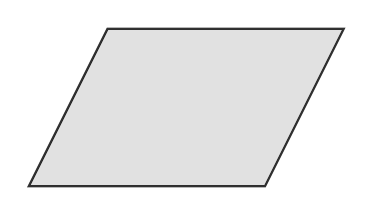
\begin{tikzpicture}
        \coordinate (A) at (0, 0);
        \coordinate (B) at (3, 0);
        \coordinate (C) at (4, 2);
        \coordinate (D) at (1, 2);
        \draw[thick, fill=gray!30, opacity=0.8] (A) -- (B) -- (C) -- (D) -- cycle;
    \end{tikzpicture}
\end{center}

Given $X = \mathbb{C}/L$, we construct an atlas using $\pi : \mathbb{C} \to \mathbb{C}/L$.

Pick $\varepsilon > 0$ s.t. $\forall p \in \mathbb{C}$, $B_{\varepsilon}(p)$ intersects each $[z]$ in at most one point.

Thus gives a homeomorphism
$$
\pi : B_{\varepsilon}(p) \xrightarrow{\cong} \pi(B_{\varepsilon}(p))
$$
$$
\text{with } \phi_p = \pi \big|_{B_{\varepsilon}(p)} : U_p \subset X
$$
where $U_p = \pi(B_{\varepsilon}(p))$.

\begin{claim*}
$$
\mathcal{A} = \{ \phi_p : U_p \to V_p \}_{p \in \mathbb{C}} \text{ is an atlas.}
$$
\end{claim*}
Compatibility of $\phi_p$ \& $\phi_q$:
Assume $U_{p, q} = U_p \cap U_q \neq \emptyset$.

The transition map is:
$$
T = \phi_q \circ \phi_p^{-1} : \phi_p(U_{p, q}) \longrightarrow \phi_q(U_{p, q})
$$
$T$ satisfies $\pi(T([z])) = \phi_p^{-1}([z]) = \pi([z])$ i.e., $T([z])-z \in L = \ker(\pi)$, which is constant.
$$
\Rightarrow T - \mathrm{id} \text{ is locally constant: locally } T - \mathrm{id} = w \in L.
$$
$$
T(z) = z + w \text{ is holomorphic}
$$
\end{enumerate}

\begin{center}
    % Placeholder for the diagram showing C mapping to X=torus
    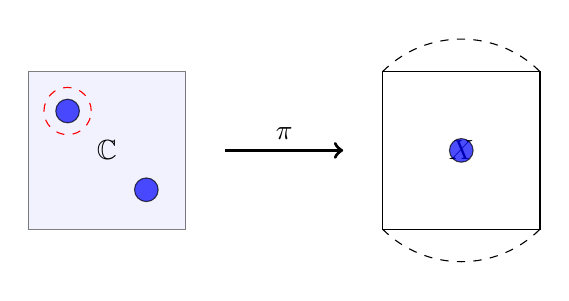
\begin{tikzpicture}
        % C plane (source)
        \draw[fill=blue!10, opacity=0.5] (-3, -0.5) rectangle (-1, 1.5);
        \node at (-2, 0.5) {$\mathbb{C}$};

        % X torus (target)
        \draw (1.5, -0.5) -- (3.5, -0.5) -- (3.5, 1.5) -- (1.5, 1.5) -- cycle;
        \draw[dashed] (1.5, 1.5) to[out=45, in=135] (3.5, 1.5);
        \draw[dashed] (1.5, -0.5) to[out=-45, in=-135] (3.5, -0.5);
        \node at (2.5, 0.5) {$X$};

        % Map pi
        \draw[->, very thick] (-0.5, 0.5) -- (1, 0.5) node[midway, above] {$\pi$};

        % Circles/points (covering map visualization)
        \draw[fill=blue, opacity=0.7] (-2.5, 1.0) circle (0.15);
        \draw[fill=blue, opacity=0.7] (-1.5, 0.0) circle (0.15);
        \draw[fill=blue, opacity=0.7] (2.5, 0.5) circle (0.15);
        \draw[dashed, red] (-2.5, 1.0) circle (0.3);
    \end{tikzpicture}
\end{center}

\subsection{Examples of complex manifolds}

\begin{example}[Complex Projective Plane]
$$
\mathbb{CP}^n = \{ \text{1-dimensional complex vector subspace in } \mathbb{C}^{n+1} \} = \mathbb{C}^{n+1} \setminus \{ 0 \} / \mathbb{C}^*.
$$
$$
\cong S^{2n+1} / S^1 \quad \text{ quotient topology.}
$$

Give $\mathbb{CP}^n$ the quotient topology.
$$
\pi : \mathbb{C}^{n+1} \setminus \{ 0 \} \longrightarrow \mathbb{CP}^n
$$
$$
(z_0, \dots, z_n) \longmapsto \pi(z_0, \dots, z_n) = [z_0 : z_1 : \dots : z_n].
$$
homogeneous coordinates.

\textbf{Atlases:}
Let
$$
U_i = \{ [z_0 : \dots : z_n] : z_i \neq 0 \} \subset \mathbb{CP}^n \quad \text{ open}
$$
The chart $\phi_i$ is given by:
$$
\phi_i : U_i \longrightarrow V_i = \mathbb{C}^n
$$
$$
[z_0 : \dots : z_n] \longmapsto \left( \frac{z_0}{z_i}, \frac{z_1}{z_i}, \dots, \widehat{\frac{z_i}{z_i}}, \dots, \frac{z_n}{z_i} \right)
$$
where $\widehat{\frac{z_i}{z_i}}$ denotes the omission of the $i$-th coordinate.
\end{example}

\section{Morphisms of complex manifolds \& meromorphic functions.}

\subsection{Morphisms of manifolds}

\begin{definition}
    Let $X$ \& $Y$ be complex \textbf{manifolds} of dimensions $n$ \& $m$ respectively.
    Let $W \subset X$ \& $W' \subset Y$ be open sets.
    \begin{enumerate}
        \item A continuous map $F: W \to W'$ is holomorphic at $p \in W$
        if $\exists$ charts $\phi : U \to V$ \& $\psi : W' \to V'$ s.t. $p \in U$
        \& $F(p) \in W'$, s.t. $\psi \circ F \circ \phi^{-1}$ is holo at $\phi(p)$.
        \item Biholomorphism.
    \end{enumerate}
\end{definition}

\begin{example}(Examples of Morphisms)
\begin{enumerate}
    \item A chart on a Riemann Surface $\phi : U \to V \subset \mathbb{C}$ on a Riemann Surface is a holomorphic function.
    \item Let $U \subset X$ for a Riemann Surface $X$. Then $U$ has a unique Riemann Surface structure s.t. the inclusion map $U \hookrightarrow X$ is holomorphic.
    \item Let $\mathbb{C}_{\infty} = \mathbb{C} \cup \{\infty\} \cong S^2 = U_0 \cup U_{\infty}$.
    Let $f$ be a holomorphic function on $\mathbb{C}$.
    Let $f_0 := f \circ \phi_0^{-1} : \mathbb{C} \to \mathbb{C}$.
    Let $f_{\infty} := f \circ \phi_{\infty}^{-1} : \mathbb{C} \to \mathbb{C}$.
On $\mathbb{C}^*$:
$$
f_{\infty}(w) = f \circ \phi_{\infty}^{-1}(w) = f \circ \phi_0^{-1} \circ \phi_0 \circ \phi_{\infty}^{-1}(w) = f_0 \left(\frac{1}{w}\right)
$$

This $f$ is holomorphic at $w \in \mathbb{C}_{\infty}$
$$
\iff f\left(\frac{1}{z}\right) \text{ is holomorphic at } 0
$$
$$
\Updownarrow \text{ Def}
$$
$$
f_{\infty}(w) \text{ is holomorphic at } 0 \iff f_0 \left(\frac{1}{w}\right) \text{ is holomorphic at } \infty
$$
 \item the quotient map $\pi: \mathbb{C}^n \to \mathbb{C}^n/L$ for a complex torus is holomorphic.
\end{enumerate}
\end{example}

subsection*{$\S$ 2.2. Properties of holomorphic maps of Riemann Surfaces.}

\begin{theorem}[The identity theorem] \label{thm:identity}
    Let $F, G: X \to Y$ be holomorphic maps of Riemann Surfaces s.t. $F$ \& $G$ agree on a subset of $X$ with an accumulation point.
    Then $F=G$.
\end{theorem}

\begin{theorem}[Local form of holomorphic maps] \label{thm:localform}
    Let $F: X \to Y$ be a non-constant holomorphic map of Riemann Surfaces.
    For $p \in X$ \& $q = F(p)$, $\exists$ unique $k \in \mathbb{Z}_{>0}$ and local charts $\phi : U \to V$ \& $\psi : U' \to V'$
    s.t. $F$ has local form
    $$
    \psi \circ F \circ \phi^{-1} : V \to V'
    $$
    $$
    z \mapsto z^k.
    $$
\end{theorem}

\begin{proof} 
    take any charts $\phi: U \to V \subset \mathbb{C}$ \& $\psi: U' \to V' \subset \mathbb{C}$.
$$
\begin{array}{ccc}
    X & \xrightarrow{F} & Y \\
    \downarrow{\phi} & & \downarrow{\psi} \\
    \mathbb{C} & \xrightarrow{f} & \mathbb{C}
\end{array}
\quad
\begin{array}{l}
    p \mapsto 0. \\
    q \mapsto 0.
\end{array}
$$

Shrink $V$ so $F(U) \subset U'$. Then $f = \psi \circ F \circ \phi^{-1} : V \to V'$
is holomorphic and $0 \mapsto 0$.

Define $k = \mathrm{ord}_0(f) \in \mathbb{Z}_{\ge 0}$. $\mathrm{ord}_0(f)$ is the order of vanishing of $f$
at $0 = \min \{ n \mid c_n \neq 0 \}$ where $f(z) = \sum_{n \ge 0} c_n z^n$ is
the Taylor expansion. $f(z) = z^k g(z)$, where $g(z)$ is non-zero.

Shrink $V$ so $g: V \to \mathbb{C}$ is non-zero and holomorphic.
Thus, $\exists$ holomorphic $k^{\text{th}}$ root $h: V \to \mathbb{C}$ of $g$
i.e., $(h(z))^k = g(z)$.

Thus $f(z) = z^k g(z) = (z h(z))^k$.

Let $\alpha : V \xrightarrow{\cong} \alpha(V)$ be biholomorphic
$$
z \mapsto z h(z) = w.
$$
Note $\alpha(0) = 0$, $\alpha'(0) = h(0) \neq 0$, then $\mathrm{ord}_0(\alpha) = 1$.

Now replace $\phi$ by $\alpha \circ \phi$.
$$
\psi \circ F \circ (\alpha \circ \phi)^{-1}(w) = \psi \circ F \circ \phi^{-1} \circ \alpha^{-1}(w)
$$
$$
= f(\alpha^{-1}(w)) = (\alpha^{-1}(w) h(\alpha^{-1}(w)))^k = w^k.
$$
Local form is $w \mapsto w^k$.
\end{proof}

\begin{exercise}
Show $k$ is independent of the choice of chart.
\end{exercise}
\begin{definition}
    The \textbf{multiplicity} of a non-constant holomorphic map $F: X \to Y$
    of Riemann Surfaces at $p \in X$ is the unique positive integer $k$ given by
    Theorem 2.2.
\end{definition}

We say $p$ is an \underline{unramified point} of $F$ if $\mathrm{mult}_p(F) = 1$.
$p$ is a \underline{ramified point} of $F$ if $\mathrm{mult}_p(F) > 1$.

$$
R(F) = \{ p \in X : \mathrm{mult}_p(F) > 1 \} \text{ ramification locus.}
$$
$$
B(F) = F(R(F)) \subset Y \text{ branch locus.}
$$

\begin{theorem}
    (Open mapping theorem) \label{thm:openmapping}
    A non-constant holomorphic map of Riemann Surfaces is an open mapping.
\end{theorem}

\textbf{Proof:} The local form $z \mapsto z^k$ is open
("maps circle to circle").

\begin{theorem}
    (Biholomorphic maps are biholomorphisms) \label{thm:biholo}
    The inverse of a bijective holomorphic map of Riemann Surfaces is holomorphic
    (since $F$ is an open mapping).
\end{theorem}

\begin{theorem}
(Discreteness of preimages)
Let $F: X \to Y$ non constant map of RS. Then $\forall q \in Y$.
the preimage $F^{-1}(q)$ is discrete in $X$.
(\textcolor{red}{If $X$ is compact then $F^{-1}(q)$ is finite})
\end{theorem}

\begin{proof}
$F$ follows as a holomorphic map of the complex plane are discrete.
\end{proof}

\begin{theorem}
(Surjectivity of non-constant holomorphic map from compact RS)
Let $F: X \to Y$ a non-constant holomorphic map of RS with $X$ compact.
Then $F$ is surjective and $Y$ is compact.
\end{theorem}

\begin{proof}
Open mapping theorem $\implies F(X) \subset Y$ is open
$F$ continuous and $X$ compact $\implies F(X)$ compact hence closed (and $Y$ hausdorff) $\square$.
\end{proof}

\begin{corollary}
Every holomorphic function on a compact Riemann Surface ($\mathbf{RS}$) is constant.
\end{corollary}
\textbf{Proof:}
Let $f: X \to \mathbb{C}$ be a non-constant holomorphic function.
Then $f$ is constant.
\hfill $\square$

\begin{theorem} [Riemann's extension theorem] 
Let $X$ be a $\mathbf{RS}$, $p \in U \subset_{\text{open}} X$. If $f: U \setminus \{p\} \to \mathbb{C}$ is holomorphic and bounded in a punctured neighborhood of $p$, then $f$ extends to a holomorphic function on $U$.
\end{theorem}
\textbf{Proof:}
Follows from complex analysis using charts.
\hfill $\square$

\begin{theorem} [Maximum principle] 
Let $f: X \to \mathbb{C}$ be a non-constant holomorphic function on a $\mathbf{RS}$ $X$.
Then $|f|$ has no local maximum.
\end{theorem}

\subsection{Meromorphic functions on Riemann Surfaces}

\begin{definition}
Let $X$ be a $\mathbf{RS}$ and $p \in W \subset_{\text{open}} X$. If $f: W \setminus \{p\} \to \mathbb{C}$ is holomorphic, we say that $p$ is a
$$
\left\{
\begin{array}{ll}
\text{removable singularity} & \\
\text{pole} &  \\
\text{essential singularity} & 
\end{array}
\right\}
\text{ if } \exists \text{ chart } \phi: U \to V , \text{ s.t. } \phi(p) \text{ is a }
\left\{
\begin{array}{l}
\text{removable singularity} \\
\text{pole} \\
\text{essential singularity}
\end{array}
\right\}
$$
We say $f$ is **meromorphic** at $p$ if $p$ is a **non-essential singularity**.

If $S \subset W \subset_{\text{open}} X$ and $f: W \setminus S \to \mathbb{C}$ is holomorphic, we say $f$ is **meromorphic** on $W$ if it is **meromorphic** at each $p \in S$.
\end{definition}

\textbf{Notation}
Let $U \subset_{\text{open}} X$.
\begin{itemize}
    \item $\mathcal{O}_X(U) = \{f: U \to \mathbb{C} \mid f \text{ is holomorphic}\}$
    \item $\mathcal{M}_X(U) = \{f: U \setminus S \to \mathbb{C} \mid f \text{ is meromorphic on } U\}$
\end{itemize}

\begin{lemma}
\begin{enumerate}[i)]
    \item The above definition is independent of the choice of chart.
    \item $\mathcal{O}(X) = \mathcal{O}_X(X)$ is a $\mathbb{C}$-algebra.
    \item $\mathcal{M}(X) = \mathcal{M}_X(X)$ is a field, called the **function field of $X$**.
    \item $\mathcal{M}(X) = \text{Frac}(\mathcal{O}(X))$.
    \item $p$ has a
    $$
    \left\{
    \begin{array}{l}
    \text{removable singularity} \\
    \text{pole} \\
    \text{essential singularity}
    \end{array}
    \right\} \text{ at } p \text{ if }
    \left\{
    \begin{array}{l}
    |f| \text{ is bounded in a neighborhood of } p \\
    \lim_{z \to p} |f(z)| = \infty \\
    \lim_{z \to p} f(z) \text{ doesn't exist}
    \end{array}
    \right\}
    $$
\end{enumerate}
\end{lemma}

\subsection{Laurent Expansions \& Orders of Singularities}
Let $f: W \setminus \{p\} \to \mathbb{C}$ be a holomorphic function with $p \in W \subset_{\text{open}} X$, where $X$ is a **Riemann Surface**.
Let $\phi: U \to V$ be a chart on $X$, such that $\phi(p) = 0$.
Then $f \circ \phi^{-1}: V \setminus \{0\} \to \mathbb{C}$ is holomorphic and has a Laurent expansion at $0$.
$$
f \circ \phi^{-1}(z) = \sum_{n = -\omega}^{\infty} c_n z^n \quad \text{(\textbf{Note}: This depends on the choice of chart.)}
$$

\begin{definition}
The **order of $f$** is defined as:
$$
\text{ord}_p(f) := \text{ord}_0(f \circ \phi^{-1}) = \min \{n \in \mathbb{Z} \mid c_n \neq 0\}
$$
If $f(z) = 0$ for all $z$, then $\text{ord}_p(0) = \infty$.
\end{definition}

\begin{lemma}
\begin{enumerate}[i)]
    \item $\text{ord}_p(f)$ is independent of the chart $\phi$ centered at $p$.
    \item $X$ is a
    $$
    \left\{
    \begin{array}{l}
    \text{removable singularity} \\
    \text{pole} \\
    \text{essential singularity}
    \end{array}
    \right\} \text{ of } f \text{ if } \text{ord}_p(f) =
    \left\{
    \begin{array}{l}
    \geq 0 \\
    -m, \quad m > 0 \quad \text{(i.e., } < 0 \text{)} \\
    -\infty
    \end{array}
    \right\}
    $$
    \item $\text{ord}_p(f^{-1}) = -\text{ord}_p(f)$.
    \item $\text{ord}_p(f g) = \text{ord}_p(f) + \text{ord}_p(g)$.
    \item $\text{ord}_p(f+g) \geq \min \{ \text{ord}_p(f), \text{ord}_p(g) \}$.
\end{enumerate}
\end{lemma}

\begin{example}
The map $\exp: \mathbb{C} \to \mathbb{C}$ is holomorphic on $\mathbb{C}$. Is it holomorphic or meromorphic on $\mathbb{C}_{\infty}$?
Consider $w=1/z$. For $f: \mathbb{C}_{\infty} \setminus \{0\} \to \mathbb{C}$ we have $\text{ord}_{\infty}(f) = \text{ord}_0(f(1/z))$.
Thus, $\exp(w)$ has an essential singularity at $w=0$, so $\exp$ is not meromorphic on $\mathbb{C}_{\infty}$.
\end{example}

\begin{example} [Meromorphic functions on $\mathbb{C}_{\infty}$]
Let $z=\phi_0: U_0 \to V_0 = \mathbb{C}$. $\text{ord}_0(z) = -1$ .
Let $P, Q \in \mathbb{C}[z]$ with $Q \not\equiv 0$. We claim $f(z) = P(z)/Q(z) \in \mathcal{M}(\mathbb{C}_{\infty})$.
We know $f \in \mathcal{M}(\mathbb{C})$: what about at $\infty$?
Let $f(z) = \lambda \prod_{i} (z-a_i)^{k_i}$, where $a_i \in \mathbb{C}$ and $k_i \in \mathbb{Z}$. $x \in \mathbb{C}$.
$f(z)$ is meromorphic at $\infty$ if $f(1/z)$ is meromorphic at $0$.
$$
f(1/z) =\lambda \prod_{i} (1/z - a_i)^{k_i} = \lambda z^{-\sum k_i} \prod_{i}  (1 - a_i z)^{k_i}
$$
$$
\text{ord}_{\infty}(f) =
\left\{
\begin{array}{ll}
-\sum k_i & p=\infty \\
k_i & p=a_i \\
0 & \text{otherwise}
\end{array}
\right.
\quad \text{Note: } \sum_{p \in \mathbb{C}_{\infty}} \text{ord}_p(f) = 0.
$$
\end{example}

\begin{theorem} [Meromorphic functions as holomorphic maps to $\mathbb{C}_{\infty}$] 
For a **Riemann Surface** $X$, there is a 1-1 correspondence:
$$
\mathcal{M}(X) = \{ \text{meromorphic functions on } X \} \longleftrightarrow \{ \text{holomorphic maps } F: X \to \mathbb{C}_{\infty} \mid F \not \equiv \infty \}
$$
The correspondence is given by:
$$
f \longmapsto F: X \to \mathbb{C}_{\infty}, \quad F(x) =
\left\{
\begin{array}{ll}
f(x), & x \notin \text{Pole}(f) \\
\infty, & x \in \text{Pole}(f)
\end{array}
\right.
$$
$$
f = \phi_{\infty} \circ F \mid_{F^{-1}(\mathbb{C})} \longleftarrow F: X \to \mathbb{C}_{\infty}.
$$
and $f(x)=\infty$ if $F(x)=\infty$.
\end{theorem}

\begin{proof}
The map $F$ associated to $f \in \mathcal{M}(X)$ is holomorphic on $X \setminus \text{Pole}(f)$.
\textbf{We want to show:} $F$ is holomorphic at each $p \in \text{Pole}(f)$.
$f$ has a pole at $p \iff f \circ \psi^{-1}$ has a pole at $\psi(p)=0$ (by definition).\\
$\iff \phi_{\infty} \circ F \circ \psi^{-1} = \frac{1}{f \circ \phi^{-1}} \text{ has a zero at } \psi(p) = 0.$
This means $F$ is holomorphic at $p$ (by definition of holomorphicity for a map to $\mathbb{C}_{\infty}$).
\end{proof}

\begin{lemma} [Relating the order of $f \in \mathcal{M}(X)$ and the multiplicity of the corresponding map $F: X \to \mathbb{C}_{\infty}$]
For $f \in \mathcal{M}(X)$ non-constant, and $F: X \to \mathbb{C}_{\infty}$ the corresponding holomorphic map at $p \in X$:
\begin{enumerate}[i)]
    \item If $f(p)=0$, then $\text{mult}_p(F) = \text{ord}_p(f)$.
    \item If $f(p)=\infty$, then $\text{mult}_p(F) = -\text{ord}_p(f)$.
    \item Otherwise, $\text{mult}_p(F) = \text{ord}_p(f - f(p))$.
\end{enumerate}
\end{lemma}

\begin{theorem} [Meromorphic functions on $\mathbb{C}_{\infty}$] 
$$\mathcal{M}(\mathbb{C}_{\infty})=\mathbb{C}(z)$$
\end{theorem}

\textbf{Proof:}
We've seen $\mathbb{C}(z) \subset \mathcal{M}(\mathbb{C}_{\infty})$. Let $f \in \mathcal{M}(\mathbb{C}_{\infty})$.
Let $p_1, p_2, \dots, p_n$ be the zeros of $f$ in $\mathbb{C} \subset \mathbb{C}_{\infty}$.
Let $g(z) := \prod_{i=1}^n (z-p_i)^{r_i}$, where $r_i = \text{ord}_{p_i}(f) \in \mathbb{Z}$.
(Note that $g(z) \in \mathbb{C}(z)$).
By construction, $\text{ord}_p(f) = \text{ord}_p(g)$ for all $p \in \mathbb{C}$. Then $h = f/g \in \mathcal{M}(\mathbb{C}_{\infty})$ has no zeros and no poles in $\mathbb{C}$.

Let $h(z) = \sum c_n z^n$ be the Taylor expansion of $h$ at $0 \in \mathbb{C}$.
Let $w = 1/z$ be a local coordinate at $\infty \in \mathbb{C}_{\infty}$. Then
$$
h(w) = \sum c_n w^{-n}
$$
is the Laurent expansion of $h$ at $\infty$.
Since $h$ is meromorphic at $\infty$, then $h(z) = \sum_{n=0}^m c_n z^n \in \mathbb{C}[z]$ (polynomial).
If $\deg(h) > 0$, then $h$ has a zero in $\mathbb{C}$. Thus $h(z) = \lambda$, a constant.
And $f = \lambda g \in \mathbb{C}(z)$.
\hfill $\square$

\begin{corollary}
For $f \in \mathcal{M}(\mathbb{C}_{\infty})$, $\sum_{p \in \mathbb{C}_{\infty}} \text{ord}_p(f) = 0$.
\end{corollary}

\subsection{The degree of a holomorphic map}

\begin{theorem} \label{degree of holo map between copt rs}
Let $F: X \to Y$ be a non-constant holomorphic map of compact **Riemann Surfaces**.
For $q \in Y$, the quantity $\text{deg}_q(F) = \sum_{p \in F^{-1}(q)} \text{mult}_p(F)$ is independent of $q$.
\end{theorem}

\begin{definition}
The **degree of $F$** is $\deg(F) = \deg_q(F)$ for any $q \in Y$.
\end{definition}

\begin{proof}
For $q \in Y$, take $F^{-1}(q) = \{p_1, p_2, \dots, p_s\}$ and let $k_i = \text{mult}_{p_i}(F)$.
By Theorem 2.2, $\exists$ local normal forms at each $p_i$, i.e.,
$\exists$ charts $\phi_i: U_i \to V_i$ on $X$ and $\psi: U_i' \to V_i'$ on $Y$,
such that $F(U_i) \subset U_i'$, $p_i \to 0$, $q \to 0$,
and $\psi \circ F \circ \phi_i^{-1}(z) = z^{k_i}$. Assume the $U_i$ are pairwise disjoint.
\begin{claim*}
$\exists$ open neighborhood $W$ of $q$ in $Y$ such that $F^{-1}(W) \subset \bigcup_{i} U_i$.
\end{claim*}
\textbf{Proof of Claim:}
Let $\overline{W}$ be an open neighborhood of $q$, $\overline{W} = \{q\} \cup \text{something else}$.
Let $W$ be an open neighborhood of $q$ such that $W \cap F(X \setminus \bigcup_i U_i) = \emptyset$.
Thus $F^{-1}(W) \cap (X \setminus \bigcup_i U_i) = \emptyset$.
Since $X$ is compact, $F(X \setminus \bigcup_i U_i)$ is compact.
$\exists$ an open neighborhood $W_i$ of $q$ in $Y$ such that $F^{-1}(W_i) \cap (X \setminus U_i) = \emptyset$.Let $W = \bigcap_{i=1}^s W_i$, which is an open neighborhood of $q$. Then $F^{-1}(W) \subset \bigcup_{i=1}^s U_i$. $\square$

For any $q' \in W$, we have $\deg_{q'}(F) = \deg_q(F)$.
This is because, for $q' \in W$, $F^{-1}(q') \cap U_i$ consists of $k_i$ points of multiplicity 1.
Hence $\deg_q(F)$ is locally constant, and as $Y$ is connected, $\deg_q(F)$ is constant.
\end{proof}

\begin{remark}
Let $f: X \to \mathbb{C}$. If $f$ is locally constant and $X$ is connected,
then $f$ is a constant.
\end{remark}

\begin{proof}
Take $p \in X$. $\exists U_p \subset X$ such that $f|_{U_p}$ is a constant $f(p)$.
Consider $\mathcal{O} = \{x \in X \mid f(x) = f(p)\}$.
\begin{enumerate}
    \item $\mathcal{O}$ is open since $f$ is locally constant.
    \item $\mathcal{O}$ is closed since $f$ is locally constant.
\end{enumerate}
If $y \in X \setminus \mathcal{O}$, then $f(y) \neq f(p)$. Then $\exists U_y$ such that $U_y \subset X \setminus \mathcal{O}$.
Since $X$ is connected and $\mathcal{O}$ is non-empty (as $p \in \mathcal{O}$) and is both open and closed, we must have $\mathcal{O} = X$.
Thus $f$ is constant.
\end{proof}

\begin{remark}
\begin{enumerate}
    \item At a ramification point $p$, $F$ looks locally like $\mathbb{C} \to \mathbb{C}, z \mapsto z^k$.
    \item $F|_{X \setminus R(F)}: X \setminus R(F) \to Y \setminus B(F)$ is a $d$-sheeted covering, where $d = \deg(F)$.
\end{enumerate}
\end{remark}

\begin{corollary}
\begin{enumerate}[i)]
    \item If $F$ is a degree 1 non-constant holomorphic map of compact **Riemann Surfaces** ($\mathbf{RS}$), then $F$ is a **biholomorphism** (surjectivity + injectivity).
    \item If $X$ is compact and has a meromorphic function with a single simple pole, then $X \cong \mathbb{C}_{\infty}$.
\end{enumerate}
\end{corollary}

\begin{proof}
    \begin{exercise}
        
    \end{exercise}
\end{proof}

\begin{corollary}
$\mathbb{C}\mathbb{P}^1 \cong \mathbb{C}_{\infty}$.
\end{corollary}

\begin{corollary}
Let $X$ be a compact **Riemann Surface** ($\mathbf{RS}$) and $f \in \mathcal{M}(X)$ non-constant.
Then $\sum_{p \in X} \text{ord}_p(f) = 0$.
\end{corollary}

\begin{proof}
Let $F: X \to \mathbb{C}_{\infty}$ be the associated holomorphic map.
We know that:
$$
\sum_{p \in X} \text{ord}_p(f) = \sum_{p \in \text{Zero}(f)} \text{ord}_p(f) + \sum_{p \in \text{Pole}(f)} \text{ord}_p(f)
$$
We use the relationship between order and multiplicity
$$
\sum_{p \in \text{Zero}(f)} \text{ord}_p(f) = \sum_{p \in F^{-1}(0)} \text{mult}_p(F)
$$
And
$$
\sum_{p \in \text{Pole}(f)} \text{ord}_p(f) = \sum_{p \in F^{-1}(\infty)} (-\text{mult}_p(F)) = -\sum_{p \in F^{-1}(\infty)} \text{mult}_p(F)
$$
Substituting these back:
$$
\sum_{p \in X} \text{ord}_p(f) = \sum_{p \in F^{-1}(0)} \text{mult}_p(F) - \sum_{p \in F^{-1}(\infty)} \text{mult}_p(F)
$$
Since $\sum_{p \in F^{-1}(q)} \text{mult}_p(F) = \deg(F)$ for any $q \in \mathbb{C}_{\infty}$:
$$
= \deg(F) - \deg(F) = 0.
$$
\end{proof}

\subsection{Germs of holomorphic functions}

\begin{definition}
For a complex manifold $X$ and $p \in X$, we define the ring of germs of holomorphic functions at $p$:
$$
\mathcal{O}_{X, p} = \left\{ (U, f) \mid U \text{ is an open neighborhood of } p, f: U \to \mathbb{C} \text{ is holomorphic} \right\} / \sim
$$
where $\sim$ is the equivalence relation defined by:
$$
(U, f) \sim (V, g) \iff \exists \text{ a neighborhood } W \text{ of } p \text{ s.t. } f|_W = g|_W
$$
The equivalence class $[(U, f)]$ is called the **germ of $f$ at $p$**.
\end{definition}

\begin{remark}
\begin{enumerate}
    \item $\mathcal{O}_{X, p}$ is a ring whose non-invertible elements form an ideal.
    \item The maximal ideal $\mathfrak{m}_p$ is given by:
    $$
    \mathfrak{m}_p = \{ [(U, f)] \mid f(p) = 0 \}. \quad (\text{germs vanishing at } p)
    $$
    This is the kernel of the evaluation map:
    $$
    \text{ker}(\text{ev}_p: \mathcal{O}_{X, p} \to \mathbb{C}).
    $$
    Thus $\mathcal{O}_{X, p} / \mathfrak{m}_p \cong \mathbb{C}$. This means $\mathfrak{m}_p$ is a **maximal ideal** (local ring).
\end{enumerate}
\end{remark}

\begin{example}
\begin{enumerate}
    \item $\mathcal{O}_{\mathbb{C}^n, 0} \cong \mathbb{C} \{x_1, \dots, x_n\}$.
    $$
    [(U, f)] \mapsto \text{Taylor expansion of } f \text{ at } 0.
    $$
    \item If $X$ is an $n$-dimensional complex manifold and $p \in X$, then a local chart $\phi: U \to V$, centered at $p$, induces an isomorphism:
    $$
    \phi^*: \mathcal{O}_{\mathbb{C}^n, 0} \to \mathcal{O}_{X, p}
    $$
    which maps the germ $[(V, \psi)]$ to the germ $[(U, \psi \circ \phi)]$.
\end{enumerate}
\end{example}

\subsection{$\mathcal{O}_{X, p}$ for a Riemann Surface}
The order of a **holomorphic** function at $p$ descends to a map
$$
\text{ord}_p: \mathcal{O}_{X, p} \to \mathbb{N} \cup \{\infty\} \text{ satisfying}
$$

\begin{enumerate}
    \setcounter{enumi}{2} % Continue from the previous list on the previous page
    \item $\text{ord}_p(f) = \infty \iff f \equiv 0$.
    \item $\text{ord}_p(f g) = \text{ord}_p(f) + \text{ord}_p(g)$.
    \item $\text{ord}_p(f+g) \geq \min \{\text{ord}_p(f), \text{ord}_p(g)\}$.
\end{enumerate}
This is known as a **discrete valuation**.

We can extend $\text{ord}_p$ to $\text{Frac}(\mathcal{O}_{X, p})$ by $\text{ord}_p(f/g) = \text{ord}_p(f) - \text{ord}_p(g)$.

\begin{lemma}
For a **Riemann Surface** $X$, $\mathcal{O}_{X, p}$ is a **Discrete Valuation Ring** ($\mathbf{DVR}$) with valuation given by $\text{ord}_p: \text{Frac}(\mathcal{O}_{X, p}) \to \mathbb{Z} \cup \{\infty\}$.
The **uniformizer** (element with valuation 1) is given by a local chart centered at $p$.
\end{lemma}

\subsection{Jacobians and the implicit function theorem}

\begin{definition}
The complex Jacobian of a holomorphic map $f: \mathbb{C}^n \to \mathbb{C}^m$ at $p \in \mathbb{C}^n$ is
$$
J_{\mathbb{C}} f(p) := \left( \frac{\partial f_j}{\partial z_k} (p) \right)_{j, k} = \begin{pmatrix}
\frac{\partial f_1}{\partial z_1} (p) & \cdots & \frac{\partial f_1}{\partial z_n} (p) \\
\vdots & \ddots & \vdots \\
\frac{\partial f_m}{\partial z_1} (p) & \cdots & \frac{\partial f_m}{\partial z_n} (p)
\end{pmatrix} \in M_{m \times n} (\mathbb{C})
$$
We say $p$ is a \textbf{regular point} of $f$ if $J_{\mathbb{C}} f(p): \mathbb{C}^n \to \mathbb{C}^m$ is surjective.
We say $q \in \mathbb{C}^m$ is a \textbf{regular value} of $f$ if all of its preimages are regular points.
\end{definition}

\begin{example}
If $n=m=1$, then $J_{\mathbb{C}} f(p) = \left( \frac{\partial f}{\partial z} (p) \right)$.
\end{example}

\textbf{Relationship with the Real Jacobian}\\
Consider $f: \mathbb{C}^n \to \mathbb{C}^m$ real differentiable.
$$
\begin{array}{ccc}
\mathbb{C}^n & \to & \mathbb{C}^m \\
\mathbb{R}^{2n} & & \mathbb{R}^{2m}
\end{array}
$$

$$
J_{\mathbb{R}} f(p) = \begin{pmatrix}
\left( \frac{\partial u_j}{\partial x_k} (p) \right)_{j, k} & \left( \frac{\partial u_j}{\partial y_k} (p) \right)_{j, k} \\
\left( \frac{\partial v_j}{\partial x_k} (p) \right)_{j, k} & \left( \frac{\partial v_j}{\partial y_k} (p) \right)_{j, k}
\end{pmatrix} \in M_{2m \times 2n} (\mathbb{R})
$$
If $f$ is holomorphic at $p$:
$$
\begin{pmatrix}
\left( \frac{\partial u_j}{\partial x_k} (p) \right)_{j, k} & \left( \frac{\partial u_j}{\partial y_k} (p) \right)_{j, k} \\
- \left( \frac{\partial u_j}{\partial y_k} (p) \right)_{j, k} & \left( \frac{\partial u_j}{\partial x_k} (p) \right)_{j, k}
\end{pmatrix}
$$

Extend coordinates from $\mathbb{R}$ to $\mathbb{C}$ and consider the change of basis:
$$
\frac{\partial}{\partial \bar{z}_k} \quad \frac{\partial}{\partial z_k}
$$
$$
\frac{\partial}{\partial z_k} = \frac{1}{2} \left( \frac{\partial}{\partial x_k} - i \frac{\partial}{\partial y_k} \right) \quad \text{and} \quad \frac{\partial}{\partial \bar{z}_k} = \frac{1}{2} \left( \frac{\partial}{\partial x_k} + i \frac{\partial}{\partial y_k} \right)
$$
In the language of manifolds, $J_{\mathbb{R}}$ is written under the basis $\frac{\partial}{\partial x_k}$ and $\frac{\partial}{\partial y_k}$.
Now we do change of basis to $\frac{\partial}{\partial z_k}$ and $\frac{\partial}{\partial \bar{z}_k}$.

$$
\left[ \frac{\partial}{\partial x_1}, \ldots, \frac{\partial}{\partial x_n}, \frac{\partial}{\partial y_1}, \ldots, \frac{\partial}{\partial y_n} \right] A = T \left[ \frac{\partial}{\partial x_1}, \ldots, \frac{\partial}{\partial x_n}, \frac{\partial}{\partial y_1}, \ldots, \frac{\partial}{\partial y_n} \right] \quad (\ast)
$$
$$
\left[ \frac{\partial}{\partial z_1}, \ldots, \frac{\partial}{\partial z_n}, \frac{\partial}{\partial \bar{z}_1}, \ldots, \frac{\partial}{\partial \bar{z}_n} \right] B = T \left[ \frac{\partial}{\partial z_1}, \ldots, \frac{\partial}{\partial \bar{z}_n} \right] \quad (\ast\ast)
$$
Also note that
$$
\left[ \frac{\partial}{\partial z_1}, \ldots, \frac{\partial}{\partial z_n}, \frac{\partial}{\partial \bar{z}_1}, \ldots, \frac{\partial}{\partial \bar{z}_n} \right] = \left[ \frac{\partial}{\partial x_1}, \ldots, \frac{\partial}{\partial x_n}, \frac{\partial}{\partial y_1}, \ldots, \frac{\partial}{\partial y_n} \right] P
$$
$$
P = \frac{1}{2} \begin{pmatrix}
I & I \\
-iI & iI
\end{pmatrix}
$$
$$
P^{-1} = 2 \begin{pmatrix}
I & iI \\
I & -iI
\end{pmatrix} \quad (\text{correct the mistake})
$$
and then plug it in we get $B = P^{-1} A P$.

With respect to this basis, $J_{\mathbb{R}} f$ has form
$$
\begin{pmatrix}
\left( \frac{\partial f_j}{\partial x_k} (p) \right)_{j, k} & \left( \frac{\partial f_j}{\partial y_k} (p) \right)_{j, k} \\
\left( \frac{\partial \bar{f}_j}{\partial x_k} (p) \right)_{j, k} & \left( \frac{\partial \bar{f}_j}{\partial y_k} (p) \right)_{j, k}
\end{pmatrix}
$$
If $f$ is holomorphic at $p$:
$$
\begin{pmatrix}
J_{\mathbb{C}} f(p) & 0 \\
0 & \overline{J_{\mathbb{C}} f(p)}
\end{pmatrix}
$$

\begin{example}
$n=m=1$
$$
P^{-1} \begin{pmatrix} u_x & u_y \\ v_x & v_y \end{pmatrix} P =
$$
\end{example}

\begin{lemma}
Suppose $n=m$ and $f: \mathbb{C}^n \to \mathbb{C}^n$ is holomorphic at $p \in \mathbb{C}^n$.
\begin{enumerate}[(i)]
    \item $\det J_{\mathbb{R}} f(p) = | \det J_{\mathbb{C}} f(p) |^2 \ge 0$.
    \item $\det J_{\mathbb{R}} f(p) \ne 0 \iff \det (J_{\mathbb{C}} f(p)) \ne 0 \iff p$ is a regular point of $f$.
\end{enumerate}
\end{lemma}

\begin{theorem}[Holomorphic inverse function theorem]
Let $F: U \to V$ be a holomorphic map of open sets $U, V \subset \mathbb{C}^n$ and let $p \in U$ be a regular point of $F$. Then there exist open sets $U' \subset U$, and $V' \subset V$ such that $p \in U'$ and $F(U') \subset V'$ and $F|_{U'} : U' \to V'$ is a holomorphism.
\end{theorem}

\begin{proof}
By the lemma, $p$ is a regular point of $F$
$$
\implies \det (J_{\mathbb{R}} F(p)) \ne 0
$$
Then by the real inverse function theorem,
$$
\exists \text{ real differentiable inverse of } F \text{ locally at } p, \text{ say } F^{-1}: V' \to U'.
$$
We need to check $F^{-1}$ is holomorphic at $p$.
$F$ is holomorphic at $p$
$$
\implies dF|_{p} : \mathbb{R}^{2n} \to \mathbb{R}^{2n} \text{ is } \mathbb{C}\text{-linear}
$$
$$
\implies dF^{-1}|_{F(p)} : \mathbb{R}^{2n} \to \mathbb{R}^{2n} \text{ is } \mathbb{C}\text{-linear}
$$
$$
\implies F^{-1} \text{ is holomorphic at } p'.
$$
\end{proof}

\begin{theorem}[Holomorphic implicit function theorem]
Let $F: U \to \mathbb{C}^m$ be holomorphic, and $p = (a, b) \in U$.
$$
U \underset{\text{open}}{\subset} \mathbb{C}^n \times \mathbb{C}^m
$$
Suppose $\det \left( J_p^w (F) \right) \ne 0$, where $J_p^w (F) = \left( \frac{\partial F_i}{\partial w_k} (p) \right)_{\substack{1 \le i \le m \\ 1 \le k \le m}}$.
Then there exist open sets $V \subset \mathbb{C}^n$ and $W \subset \mathbb{C}^m$, $(a, b) \in V \times W \subset U$, and a holomorphic function $g: V \to W$ such that
$$
\{ (z, w) \in V \times W \mid F(z, w) = F(a, b) \} = \text{Graph}(g).
$$
i.e., locally the fibre of $F$ at $F(a, b)$ is the graph of the holomorphic function $g$.
\end{theorem}

\begin{proof}
Same as in the real case, except we use the holomorphic inverse theorem.
\end{proof}

\newpage
\section{Algebraic Curves as Riemann Surfaces}

\begin{example}
(\textbf{Motivating Example}) \\
For $f: \mathbb{C} \to \mathbb{C}$ holomorphic, $\text{Graph}(f) = \{ (z, w) \in \mathbb{C}^2 \mid f(z) = w \}$ is a \textbf{Riemann Surface} with charts given by $\pi_z: \text{Graph}(f) \xrightarrow{\cong} \mathbb{C}$.
\end{example}

\subsection{Affine plane curves}

\begin{definition}
A \textbf{complex affine curve} is the zero locus of non-constant $f \in \mathbb{C}[z, w]$.
$$
X := V(f) = \{ (z, w) \in \mathbb{C}^2 \mid f(z, w) = 0 \} \subset \mathbb{C}^2.
$$
\end{definition}

\begin{remark}
By the holomorphic inverse function theorem: for $p \in X$.
\begin{itemize}
    \item If $\frac{\partial f}{\partial w} (p) \ne 0$, then locally at $p$, $X$ is graph of a holomorphic function $g(z) = w$.
    \item If $\frac{\partial f}{\partial z} (p) \ne 0$, then locally at $p$, $X$ is the graph of a holomorphic function $h(w) = z$.
\end{itemize}
\end{remark}

\begin{definition}[Singular points]
Let $f \in \mathbb{C}[z, w]$ and $X = V(f)$, and $p \in X$.
\begin{enumerate}[(i)]
    \item $f$ is
    $$
    \begin{cases}
    \text{non-singular at } p & \text{if } \frac{\partial f}{\partial z} (p) \ne 0 \text{ or } \frac{\partial f}{\partial w} (p) \ne 0 \\
    \text{singular at } p & \text{if } \frac{\partial f}{\partial z} (p) = \frac{\partial f}{\partial w} (p) = 0.
    \end{cases}
    $$
    \item $X$ is \textbf{non-singular} or \textbf{smooth} if $f$ has no singular points.
\end{enumerate}
\end{definition}

\begin{definition}[Multiplicity of $p \in X = V(f)$]
At $p = (a, b) \in X = V(f)$, we have the Taylor Expansion
$$
f(z, w) = \sum_{n \ge 0} \frac{1}{n!} \sum_{k=0}^n \binom{n}{k} C_{k, n-k} (z-a)^k (w-b)^{n-k}
$$
where $C_{k, n-k} = \frac{\partial^n f}{\partial z^k \partial w^{n-k}} (p)$.

Let $\text{mult}_p(X) = \min \{ n \ge 0 : \exists k \text{ with } C_{k, n-k} \ne 0 \} \ge 1$.
If $\text{mult}_p(X) = n > 1$, we say $p$ is an \textbf{$n$-fold point} of $X$.
\end{definition}

\begin{remark}
$\text{mult}_p(X) > 1 \iff \frac{\partial f}{\partial z} (p) = \frac{\partial f}{\partial w} (p) = 0 \iff p$ is a singular point.
\end{remark}

\begin{definition}[Tangent lines]
Let $p = (a, b) \in X = V(f) \subset \mathbb{C}^2$ be a smooth point. The \textbf{tangent line} of $X$ at $p$ is the line
$$
\frac{\partial f}{\partial z} (p) (z-a) + \frac{\partial f}{\partial w} (p) (w-b) = 0.
$$
\end{definition}

\begin{theorem} \label{planecurvesaresurfaces}
If $f(z, w) \in \mathbb{C}[z, w]$ is non-singular, then the associated smooth affine plane curve $X = V(f) \subset \mathbb{C}^2$ is a Riemann surface.
(But may not be compactified.)
\end{theorem}

\begin{proof}
$\forall p \in X$:
$$
\text{i) } \frac{\partial f}{\partial z} (p) \ne 0 \quad \text{or} \quad \text{ii) } \frac{\partial f}{\partial w} (p) \ne 0.
$$
By the holomorphic implicit function theorem: $\exists$ holomorphic function $g: V_p \to W_p$,
for $V_p, W_p \subset \mathbb{C}$ and an open neighborhood $U_p \subset X$ such that
\begin{enumerate}[(i)]
    \item $W_p \times V_p \subset U_p$.
    \item $V_p \times W_p \subset U_p$.
\end{enumerate}
and $\quad \text{(i) } g_p(w) = z \quad \text{or} \quad \text{(ii)} g_p(z) = w.$
$$
\text{Consider} \quad \text{(i) } \pi_w : U_p \to \mathbb{C}, \quad \text{(ii) } \pi_z : U_p \to \mathbb{C}.
$$
$$
(z, w) \mapsto w \quad (z, w) \mapsto z.
$$
We define a chart $\phi_p: U_p \xrightarrow{\cong} \pi_{w/z}(U_p)$.

\begin{claim*}
$\mathcal{A} = \{ \phi_p \mid p \in X \}$ is an atlas.
\end{claim*}

We only have to show the compatibility. We only consider the hard case. $\phi_p = \pi_w$ and $\phi_q = \pi_z$, for $s \in U_p \cap U_q$.
One partial derivative of $f$ is non-zero at $s$.
Without loss of generality, $\frac{\partial f}{\partial w} (s) \ne 0$. $\implies \exists$ holomorphic $h: V_s \to W_s$ such that $w = h(z)$.
$$
\pi_w \circ \pi_z^{-1} : \pi_z (U_p \cap U_q) \cap V_s \to \pi_w (U_p \cap U_q) \cap W_s
$$
$$
z \longmapsto \pi_w \circ \pi_z^{-1} (z) = \pi_w (z, h(z)) = h(z)
$$
which is holomorphic.
\end{proof}

\begin{remark}
\begin{enumerate}[(i)]
    \item $X = V(f)$ is not compact.
    (Since $\pi_z$ has non-constant holomorphic functions, and $X$ has only constant holomorphic functions if $X$ is compact).
    \item \textbf{Algebraic Geometry}: If $f$ is irreducible $\implies V(f)$ is connected.
\end{enumerate}
\end{remark}

\textbf{Assume}: $f$ is irreducible, so $V(f)$ is connected.

\subsection{Projective Plane Curve}

\textbf{Motivation}: We want to compactify affine plane curves.

\textbf{Idea}:
$$
\mathbb{C}^2 \hookrightarrow \mathbb{C} P^2
$$
$$
(x, y) \mapsto [x: y: 1]
$$

\begin{definition}
A \textbf{complex projective plane curve} is the zero locus of a homogeneous polynomial $F \in \mathbb{C}[x, y, z]$ in the projective plane $\mathbb{C} P^2$.
$$
V(F) = \{ [x: y: z] \in \mathbb{C} P^2 \mid F(x, y, z) = 0 \}.
$$
\end{definition}

\textbf{From affine to projective}: homogenization and dehomogenization
$$
\mathbb{C} P^2 = \bigcup_{i=0}^2 U_i, \quad U_i \cong \mathbb{C}^2. \quad U_0 = \{ x \ne 0 \}, \quad U_1 = \{ y \ne 0 \}, \quad U_2 = \{ z \ne 0 \}.
$$

$$
\{ \text{projective plane curves} \} \longleftrightarrow \{ \text{affine plane curves} \}.
$$

$X = V(F) \subset \mathbb{C} P^2$
$$
= \bigcup_{i=0}^2 X_i \quad \implies \quad X_i = U_i \cap X \subset \mathbb{C}^2.
$$
Example: $X_2 = U_2 \cap X = V(f)$, $f(x, y) = F(x, y, 1)$.
$$
F(x, y, z) = \sum_{i+j+k=d} a_{i, j, k} x^i y^j z^k
\longleftarrow \longrightarrow
f(x, y) = \sum_{i+j \le d} a_{i, j, d-i-j} x^i y^j
$$
$$
V(F) \cap X_z = V(f).
$$

\begin{definition}
A projective plane curve $X = V(F) \subset \mathbb{C} P^2$ is \textbf{singular} at $p$ if
$$
\frac{\partial F}{\partial x} (p) = \frac{\partial F}{\partial y} (p) = \frac{\partial F}{\partial z} (p) = 0.
$$
Otherwise $p$ is \textbf{non-singular}. $X$ is \textbf{smooth} if it's smooth at every $p \in X$.
\end{definition}

\begin{exercise}
$X$ smooth $\iff X_i = X \cap U_i \subset \mathbb{C}^2$ is smooth. $\forall 0 \le i \le 2$.
\end{exercise}

\begin{theorem} \label{projplanecurvesarers}
A smooth projective plane curve $X = V(F) \subset \mathbb{C} P^2$ is a \textbf{compact Riemann Surface}.
\end{theorem}

\begin{proof}

We cover the complex projective plane $\mathbb{C}P^2$ with its three standard affine charts:
\begin{itemize}
    \item $U_0 = \{[Z_0:Z_1:Z_2] \mid Z_0 \neq 0\}$, with affine coordinates $(x,y) = (Z_1/Z_0, Z_2/Z_0)$.
    \item $U_1 = \{[Z_0:Z_1:Z_2] \mid Z_1 \neq 0\}$, with affine coordinates $(u,v) = (Z_0/Z_1, Z_2/Z_1)$.
    \item $U_2 = \{[Z_0:Z_1:Z_2] \mid Z_2 \neq 0\}$, with affine coordinates $(s,t) = (Z_0/Z_2, Z_1/Z_2)$.
\end{itemize}
Let $X_i = X \cap U_i$ for $i=0,1,2$. Each $X_i$ is a smooth affine plane curve. From a previous theorem, we know that a smooth affine curve is a Riemann surface.

We construct an atlas for $X$ by taking the union of the atlases for the Riemann surfaces $X_0, X_1,$ and $X_2$. We only need to check that the transition maps between charts from different affine pieces are holomorphic.

Consider the transition from a chart on $X_0$ to one on $X_1$. The coordinate change from $U_0$ to $U_1$ is given by:
$$ u = \frac{Z_0}{Z_1} = \frac{1}{x}, \quad v = \frac{Z_2}{Z_1} = \frac{y}{x} $$
This map is a biholomorphism on the overlap $U_0 \cap U_1$. A transition map for the atlas of $X$ is a composition of a local chart map (a projection), the coordinate change map above, and another local chart map. Since all of these maps are holomorphic, their composition is holomorphic. The same logic applies to all other pairs of affine charts.

Thus, the union of the atlases for the $X_i$ forms a valid complex atlas for $X$, making it a \textbf{Riemann Surface}.
.
\end{proof}


\subsection{Algebraic varieties (affine \& projective)}
Affine space $\mathbb{A}_{\mathbb{C}}^n := \mathbb{C}^n$ with the \textbf{Zariski topology}: where closed sets are algebraic subsets.

There are maps
$$
\{ \text{aly subsets of } \mathbb{A}_{\mathbb{C}}^n \} \underset{V}{\overset{I}{\longleftrightarrow}} \{ \text{ideals } I \subset \mathbb{C}[z_1, \ldots, z_n] \}
$$
$$
X \in \mathbb{A}_{\mathbb{C}}^n \quad \longrightarrow \quad I(X) = \{ f : f|_X = 0 \}
$$
$$
V(J) = V(f_1, \ldots, f_n) \quad \longleftarrow \quad J = \langle f_1, \ldots, f_n \rangle
$$
This is not a bijective map. Roughly the take-away message is that we have a way to move between algebra and geometry.

\begin{definition}
An \textbf{affine algebraic variety} is an algebraic subset $X \in \mathbb{A}_{\mathbb{C}}^n$ such that $I(X)$ is prime.
\begin{itemize}
    \item The \textbf{coordinate ring} of $X$ is $\mathbb{C}[z_1, \ldots, z_n] / I(X)$.
    \item The \textbf{function field} of $X$ is $\mathbb{C}(X) = \text{Frac} (\mathbb{C}[X])$.
    \item At $p = (a_1, \ldots, a_n) \in \mathbb{A}_{\mathbb{C}}^n$, $\mathfrak{m}_p = \langle z_1 - a_1, \ldots, z_n - a_n \rangle \subset \mathbb{C}[z_1, \ldots, z_n]$ is a \textbf{maximal ideal}.
    \item $\mathcal{O}_{X, p}^{\text{alg}} := \mathbb{C}[X]_{\mathfrak{m}_p} = \left\{ \frac{f}{g} : f, g \in \mathbb{C}[X] \text{ such that } g(p) \ne 0 \right\}$.
\end{itemize}
Unlike for complex manifolds, we have $\mathcal{O}_{X, p}^{\text{alg}} \ne \mathcal{O}_{X, p}^{\text{holo}}$ in general.
\end{definition}

\begin{definition}[Dimension \& smoothness]
For $p \in X = V(f_1, \ldots, f_m) \subset \mathbb{C}^n$, the \textbf{Jacobian} of $X$ at $p$ is
$$
J_{X, p} = \left( \frac{\partial f_i}{\partial z_j} (p) \right)_{i, j} \quad \text{w.r.t. to generators } f_1, \ldots, f_m.
$$
\begin{enumerate}[(i)]
    \item $\dim(X) = \min_{p \in X} \{ n - \text{rank} J_{X, p} \}$. \textbf{Dimension} of $X$.
    If $\dim(X) = 1$, we call $X$ a \textbf{curve}.
    \item $p \in X$ is \textbf{smooth} if $\dim(X) = n - \text{rank} J_{X, p}$.
    (Singular otherwise). $X$ is smooth if all $p \in X$ are smooth.
\end{enumerate}
\end{definition}

\begin{remark}
$\text{rank } J_{X, p}$ is independent of choice of generators. (Why?)
\end{remark}

\subsection{Projective algebraic curves}

Projective space $\mathbb{C} P^n$ has \textbf{Zariski topology}: where closed sets are again algebraic sets. $V(\{ F_i \mid i \in I \})$ where $F_i \in \mathbb{C}[x_0, \ldots, x_n]$ are homogeneous.
$$
V(\{ F_i \mid i \in I \}) = \{ [x_0: \ldots: x_n] \in \mathbb{C} P^n : F_i(x_0, \ldots, x_n) = 0, \forall i \in I \}.
$$

There are (non-bijective) maps
$$
\{ \text{alg subsets in } \mathbb{C} P^n \} \underset{V}{\overset{I}{\longleftrightarrow}} \{ \text{homo. ideals in } \mathbb{C}[x_0, \ldots, x_n] \}.
$$

\begin{definition}
A \textbf{projective algebraic variety} is an algebraic subset $X \subset \mathbb{C} P^n$ such that $I(X)$ is prime.
\end{definition}

\textbf{(De)homogenization: from proj to affine \& back}\\
We can do the same as before.

\begin{definition}
For $X = V(F_1, \ldots, F_m) \subset \mathbb{C} P^n$
\begin{itemize}
    \item The \textbf{homogeneous coordinate ring} of $X$ is $\mathbb{C}[x_0, \ldots, x_n] / I(X)$.
    \item The \textbf{function field} of $X = \text{function field of } X_i \text{ for any } i$.
    \item The \textbf{algebraic local ring} of $X$ at $p$ is $\mathcal{O}_{X, p}^{\text{alg}} := \mathcal{O}_{X_i, p}^{\text{alg}} \text{ for } p \in X_i$.
\end{itemize}
\end{definition}

\begin{definition}[Smoothness \& Dimensions]
$p \in X$. The \textbf{Jacobian} $J_{X, p} = \left( \frac{\partial F_i}{\partial x_j} (p) \right)_{i, j}$
\end{definition}

\begin{enumerate}[(i)]
    \item $\dim(X) = \min_{p \in X} \{ n - \text{rank} J_{X, p} \}$. If $\dim(X) = 1$, $X$ a curve.
    \item $p \in X$ smooth if $\dim(X) = n - \text{rank} J_{X, p}$, otherwise $p$ is singular.
    \item $X$ is smooth if all $p \in X$ smooth.
\end{enumerate}

\begin{exercise}
$X \subset \mathbb{C} P^n$ is smooth $\iff X_i \in \mathbb{A}_{\mathbb{C}}^n$ is smooth $\forall 0 \le i \le n$.
\end{exercise}

\begin{theorem} \label{curvesaresurfaces}
\text{(Generalized Version for the Plane Curve Version)}
\begin{enumerate}[1.]
    \item Smooth affine curves are Riemann Surfaces.
    \item Smooth projective curves are compact Riemann Surfaces.
\end{enumerate}
\end{theorem}

\begin{proof}[Proof of 1.]
Let $X = V(f_1, \ldots, f_m) \subset \mathbb{A}_{\mathbb{C}}^n$ be a smooth affine curve.
To define a complex structure on $X$, we define local charts at each $p \in X$.
$X$ smooth of $\dim 1 \implies \forall p \in X$, $J_{X, p} : \mathbb{C}^n \to \mathbb{C}^m$ has rank $n-1$.
After a change of coordinates, we can assume without loss of generality that $\frac{\partial f_i}{\partial z_j} (p)|_{j \in \{ 1, \ldots, n \}} \ne 0$.
The holomorphic implicit function theorem $\implies$ locally at $p$,
$$
X = \text{Graph}(g), \quad g: \mathbb{C} \to \mathbb{C}^{n-1}.
$$
Then $\pi_{z_1}: X \to \mathbb{C}$ is a homeomorphism onto its image and this defines a local chart $\phi_p$ at $p$.\\
\noindent As for compatibility of charts,we do the same as in the proof of  \ref{planecurvesaresurfaces}

\end{proof}
\begin{proof}[Proof of 2.]
    Note that $X=\cup X_i$, with $X_i=U_i \cap X$ are affine curves, then we proceed as the proof in \ref{projplanecurvesarers}
\end{proof}

\subsection{Holomorphic \& Meromorphic Functions on Smooth Curves}

\begin{itemize}
    \item \textbf{Smooth affine curves}
    \begin{itemize}
        \item $X = V(f_1, \dots, f_m)$ for $f_i$ poly in $\mathbb{A}^n$.
        \item $X$ is a non-compact RS (Riemann Surface).
        \item The coordinate functions $x_i$ are \textbf{holomorphic}.
        \item Any poly $g(x_1, \dots, x_n) \in \mathcal{O}(X)$.
        \item Any ratio $\frac{g(x_1, \dots, x_n)}{h(x_1, \dots, x_n)}$ of polynomials with $h \notin I(X)$ is a \textbf{meromorphic} function on $X$.
    \end{itemize}
\end{itemize}

\begin{itemize}
    \item \textbf{Smooth Projective curves}
    \begin{itemize}
        \item $X = V(F_1, \dots, F_m)$ for homogeneous $F_i$ in $\mathbb{P}^n$.
        \item $X$ is a \textbf{compact} RS.
        \item $X$ is compact $\implies \mathcal{O}(X) = \mathbb{C}$.
        \item Let $G, H \in \mathbb{C}[x_1, \dots, x_{n+1}]$ be homogeneous polynomials of the same degree.
        \item $G/H: \mathbb{P}^n \setminus V(H) \to \mathbb{C}$
        \item If $H \notin I(X)$, then $G/H \in \mathcal{M}(X)$.
    \end{itemize}
\end{itemize}

\newpage
\section{Divisors on Riemann Surfaces}

\subsection{Divisors, principal divisors and the class group.}

\begin{definition}
    \begin{enumerate}[(i)]
        \item A \textbf{divisor} on a Riemann Surface $X$ is a function
        $$D: X \to \mathbb{Z}$$
        whose support $\text{supp}(D) = \{x \in X: D(x) \neq 0\}$ is \textbf{discrete}.
        \item A divisor $D$ is \textbf{effective} ($D \ge 0$) if $\text{Im}(D) \subseteq \mathbb{N}$.
    \end{enumerate}
\end{definition}

\noindent \textbf{Notation}
    \begin{itemize}
        \item $D = \sum_{x \in X} m_x \cdot x$ with $m_x \in \mathbb{Z}$.
        \item $\text{Div}(X)$ $\coloneqq$ set of divisors on $X$.
    \end{itemize}

\begin{remark}
    $\text{Div}(X)$ is an \textbf{abelian group} under pointwise addition
    $$\sum_{x \in X} m_x \cdot x + \sum_{x \in X} n_x \cdot x = \sum_{x \in X} (m_x + n_x) \cdot x$$
    with identity the \textbf{zero-divisor}.
\end{remark}

\begin{example}
    For any $p \in X$, there is an associated divisor $\tau_p \coloneqq 1 \cdot p$.
\end{example}

\begin{definition}
    For a \textbf{compact} RS $X$, we define
    $$\text{deg}: \text{Div}(X) \to \mathbb{Z}$$
    $$D = \sum_{x \in X} m_x \cdot x \mapsto \sum_{x \in X} m_x = \deg(D)$$
\end{definition}

\begin{remark}
    $\deg$ is a \textbf{group homomorphism}.
\end{remark}

\begin{definition}
    \begin{enumerate}[(i)]
        \item The \textbf{divisor of a meromorphic function} $f \in \mathcal{M}(X)^\times$ is
        $$\text{div}(f) \coloneqq \sum_{p \in X} \text{ord}_p(f) \cdot p \in \text{Div}(X).$$
        \item $D \in \text{Div}(X)$ is \textbf{principal} if there exists $f \in \mathcal{M}(X)^\times$ such that
        $$D = \text{div}(f).$$
    \end{enumerate}
\end{definition}

\noindent \textbf{Notation:}\\
    $P\text{Div}(X) \subset \text{Div}(X)$ subset of principal divisors.


\begin{remark}
    \begin{enumerate}[(i)]
        \item $\text{div}(f)$ is a divisor with support $\text{supp}(\text{div}(f)) = Z(f) \cup P(f)$ (zeros and poles of $f$).
        \item For $X$ compact, $\deg(\text{div}(f)) = \sum_{p \in X} \text{ord}_p(f) = 0$.
        \item $\text{div}: \mathcal{M}(X)^\times \to \text{Div}(X)$ is a group homomorphism.
        \item $\text{div}(f) = \text{div}_0(f) - \text{div}_\infty(f)$ where
        $$\text{div}_0(f) = \sum_{p \in Z(f)} \text{ord}_p(f) \cdot p$$
        $$\text{div}_\infty(f) = \sum_{p \in P(f)} -\text{ord}_p(f) \cdot p$$
    \end{enumerate}
\end{remark}

\begin{example}
    \begin{enumerate}[(a)]
        \item If $f = \lambda \in \mathcal{M}(X)^\times$ is a constant function, then $\text{div}(\lambda) = 0$.
        \item If $f(z) = \lambda \prod_{i=1}^m (z-a_i)^{n_i} \in \mathbb{C}(z) = \mathcal{M}(\mathbb{C} \cup \{\infty\})$, then
        $$\text{div}(f) = \sum_{i=1}^m n_i \cdot a_i - \left(\sum_{i=1}^m n_i\right) \cdot \infty.$$
    \end{enumerate}
\end{example}

\begin{lemma}
    $P\text{Div}(X) \subset \text{Div}(X)$ is a subgroup.
\end{lemma}
\begin{proof}
    $\text{div}(fg^{\pm 1}) = \text{div}(f) \pm \text{div}(g)$.
\end{proof}

\begin{definition}
    \begin{enumerate}[(i)]
        \item Two divisors $D, E \in \text{Div}(X)$ are \textbf{linearly equivalent}, written $D \sim E$,
        if $E - D \in P\text{Div}(X)$.
        \item The \textbf{class group} of $X$ is
        $$\text{Cl}(X) = \text{Div}(X) / P\text{Div}(X) = \text{Div}(X) / \sim.$$
    \end{enumerate}
\end{definition}

\begin{remark}
    $\sim$ is an equivalence relation and $D \sim 0 \iff D \in P\text{Div}(X)$.
\end{remark}

\begin{lemma}
    For $X$ compact, $D \sim E$ then $\deg(D) = \deg(E)$.
    Thus $\deg: \text{Div}(X) \to \mathbb{Z}$ factors via $\text{Cl}(X)$.
\end{lemma}
\begin{proof}
    $D - E$ is Principal and Principal divisors have degree $0$.
\end{proof}

\begin{example}
    \begin{enumerate}[(a)]
        \item If $f \in \mathcal{M}(X)$, $\text{div}(f) \sim 0$ but $\text{div}(f) \neq 0$.
        \item Let $X = \mathbb{C} \cup \{\infty\} = \mathbb{P}^1$. Any two points $p, q \in \mathbb{C} \cup \{\infty\}$ are linearly equivalent.
        $$p - q = \text{div} \left(\frac{z - p}{z - q}\right) \quad \text{if } p, q \neq \infty.$$
    \end{enumerate}
\end{example}

\begin{lemma}
    $$\deg: \text{Cl}(\mathbb{P}^1) \to \mathbb{Z}$$
    is an \textbf{isomorphism}.
\end{lemma}

\begin{proof}
    Clearly $\deg$ is surjective. For injectivity, we claim
    $$D \in P\text{Div}(\mathbb{P}^1) \iff \deg(D) = 0.$$
    We've seen $(\implies)$. For $(\impliedby)$, take $D = \sum_{i} n_i \cdot a_i + n_{\infty} \cdot \infty$.
    $$\deg(D) = 0 \implies n_{\infty} = - \sum n_i \implies D = \text{div}\left( \prod_i (z-a_i)^{n_i} \right).$$
\end{proof}

\subsection{Pullbacks of divisors.}

\begin{definition}
    For a \textbf{non-constant holomorphic map} $F: X \to Y$ of RS, we define the \textbf{pullback map} $F^*: \text{Div}(Y) \to \text{Div}(X)$ by
    $$D = \sum_{q \in Y} n_q \cdot q \mapsto F^*(D) = \sum_{q \in Y} n_q \cdot \sum_{p \in F^{-1}(q)} \text{mult}_p(F) \cdot p$$
    $$= \sum_{p \in X} \text{mult}_p(F) \cdot n_{F(p)} \cdot p$$
\end{definition}

\begin{example}
    Recall $f \in \mathcal{M}(X)$. Corresponds to $F: X \to \mathbb{P}^1$.
    $$\text{div}_0(f) = F^*([0]) \quad \& \quad \text{div}_\infty(f) = F^*([\infty]) \quad \& \quad \text{div}(f) = F^*([0] - [\infty]).$$
\end{example}

\begin{lemma}
    \begin{enumerate}[(i)]
        \item $F^*$ is a group homomorphism.
        \item $F^*(\text{div}(g)) = \text{div}(F^*g)$ for $g \in \mathcal{M}(Y)$
        $$\text{where } F^*: \mathcal{M}(Y) \to \mathcal{M}(X)$$
        $$g \mapsto F^*g = g \circ F.$$
        \item $D_1 \sim D_2 \text{ in } \text{Div}(Y) \implies F^* D_1 \sim F^* D_2 \text{ in } \text{Div}(X)$
        i.e. $F^*$ descends to the class group.
        \item If $X$ and $Y$ are compact, then $\deg(F^*(D_1)) = \deg(D_1) \cdot \deg(F)$.
    \end{enumerate}
\end{lemma}
    \begin{exercise}
        Prove the above lemma
    \end{exercise}


\begin{example}
    If $F: X \to \mathbb{C} \cup \{\infty\}$ is holomorphic, for any $p, q \in \mathbb{C} \cup \{\infty\}$ we have $F^*([p] - [q]) \sim 0$.
\end{example}

\subsection{Intersection divisors}

Fix a smooth projective algebraic curve $X \subset \mathbb{P}^n$.

\begin{definition}
    The \textbf{intersection divisor} of $X$ with a hypersurface
    $V(G) \subset \mathbb{P}^n$ defined by a homogeneous polynomial $G \in \mathbb{C}[x_0, \dots, x_n]$
    with $G \notin I(X)$ is
    $$\text{div}_X(G) := \sum_{p \in X} \text{ord}_p(G) \cdot p \in \text{Div}(X)$$
    where
    $$\text{ord}_p(G) := \text{ord}_p(G/H)$$
    where $H \in \mathbb{C}[x_0, \dots, x_n]_{\deg(G)}$ is a homogeneous polynomial of the same degree as $G$ and $H(p) \neq 0$.

    If $\deg(G) = 1$, then we call $\text{div}_X(G)$ a \textbf{hyperplane divisor}.
    i.e. $V(G) \subset \mathbb{P}^n$ is a hyper plane.
\end{definition}

\begin{remark}
    People may wonder why we have to define $\text{ord}_p(G)$ as $\text{ord}_p(G/H)$, it is because G is not a well defined function on the projective curves, but once we we divide the $H$ we get a well-defined meromorphic functions on the projective curves (as a Riemann Surface), and hence the $\text{ord}_p$ make sense. Also, We need to check the definitnoin is independent of choice of $H$.
\end{remark}

\begin{exercise}
    Check $\text{div}_X(G)$ is well-defined.
\end{exercise}

\begin{lemma}
    If $G_1, G_2 \in \mathbb{C}[x_0, \dots, x_n]_{\deg(G)}$ with $G_1, G_2 \notin I(X)$,
    for $X \subset \mathbb{P}^n$, then $\text{div}_X(G_1) \sim \text{div}_X(G_2)$.
\end{lemma}
\begin{proof}
    $f = G_1/G_2 \in \mathcal{M}(X)$. $\text{div}(f) = \text{div}_X(G_1) - \text{div}_X(G_2)$.
\end{proof}

\begin{definition}
    The \textbf{degree of a smooth projective curve} $X \subset \mathbb{P}^n$
    is $\deg(X) = \deg(\text{div}_X(G))$ for any homogeneous polynomial of degree 1 $G \in \mathbb{C}[x_0, \dots, x_n]$
    with $G \notin I(X)$.
\end{definition}

\begin{exercise}
    For a smooth projective plane curve $X = V(F) \subset \mathbb{P}^2$
    we have $\deg(X) = \deg(F)$.
\end{exercise}

Now we are going to prove Bézout's theorem.

\begin{proposition}
For $G \in k[x_0, \ldots, x_n]_d$ with $G \notin I(X)$, for $X \subseteq \mathbb{P}^n$.
Then $\deg(\mathrm{div}_X(G)) = \deg(X)\deg(G)$.
\end{proposition}

\begin{proof}
Let $H \in k[x_0, \ldots, x_n]_d$, then $H^e \in k[x_0, \ldots, x_n]_{de}$.

By the lemma $\mathrm{div}_X(G) \sim \mathrm{div}_X(H^e) = e \cdot \mathrm{div}_X(H)$.

Thus $\deg(\mathrm{div}_X(G)) = e \cdot \deg(\mathrm{div}_X(H)) = \deg(G)\deg(X)$.
\end{proof}

\begin{corollary}[Bézout's theorem]
For smooth projective plane curves, $X=V(F)$ and $Y=V(G) \subseteq \mathbb{P}^2$.
$$ \#(X \cap Y) = \deg(\mathrm{div}_X(G)) = \deg(X)\deg(G) = \deg(Y)\deg(X) $$
or
$$ = \deg(F)\deg(G) \quad (\text{by the exercise above}) $$
\end{corollary}

\subsection*{4.4 Spaces of meromorphic functions bounded by a divisor.}

\begin{definition}
For $D = \sum_{p \in X} m_p \cdot p \in \mathrm{Div}(X)$, the space of meromorphic functions bounded by $D$ is
$$ \mathcal{L}(D) := \{0\} \cup \{ f \in \mathcal{M}(X) : \mathrm{div}(f)+D \ge 0 \} $$
$$ = \{ f \in \mathcal{M}(X) : \mathrm{ord}_p(f) + m_p \ge 0, \ \forall p \in X \} $$
\end{definition}

\begin{remark}
If $m_p > 0 \implies f$ can have a pole at $p$ of order $\le m_p$. \\
If $m_p < 0 \implies f$ can have a zero at $p$ of order $\ge -m_p$.\\
That is, $\mathcal{L}(D)$ is the space of all meromorphic fucntion that is somehow bounded in the sense of its order of zeros and poles is bounded.
\end{remark}

\begin{lemma}
(i) $\mathcal{L}(D)$ is a $\mathbb{C}$-vector space.
(ii) If $D_1 \le D_2$, then $\mathcal{L}(D_1) \subseteq \mathcal{L}(D_2)$.
(iii) $\mathcal{L}(0) = \mathcal{O}(X)$.
\end{lemma}

\begin{exercise}
    Prove the above lemma
\end{exercise}

\begin{definition}
$l(D) := \dim \mathcal{L}(D) \in \mathbb{N} \cup \{0\}$.
\end{definition}

\begin{example}
If $D \ge 0$, then $l(D) \ge 1$ as $\mathbb{C} \subseteq \mathcal{L}(D)$.
\end{example}

\begin{lemma}
If $D \sim E$, then $\mathcal{L}(D) \cong \mathcal{L}(E)$.
\end{lemma}

\begin{proof}
Write $E = D + \mathrm{div}(g)$ for $g \in \mathcal{M}(X)^\times$ and consider
$$ \mu_g : \mathcal{L}(E) \to \mathcal{L}(D) $$
$$ f \mapsto f \cdot g $$
It's well-defined since $\mathrm{div}(f \cdot g) = \mathrm{div}(f) + \mathrm{div}(g)$
$$ \mathrm{div}(f) + E \ge 0 \iff \mathrm{div}(f) + D + \mathrm{div}(g) \ge 0 $$
Thus $\mathrm{div}(f \cdot g) + D \ge 0$.

Thus is an isomorphism since $\mu_{g^{-1}} : \mathcal{L}(D) \to \mathcal{L}(E)$.
\end{proof}

\begin{lemma}
For a compact Riemann Surface $X$, and $D \in \mathrm{Div}(X)$ we have
\begin{enumerate}[(i)]
    \item $\deg(D) < 0 \implies l(D) = 0$.
    \item $\deg(D) = 0 \implies l(D) = \begin{cases} 1 & \text{if } D \text{ is principal} \\ 0 & \text{otherwise} \end{cases}$
\end{enumerate}
\end{lemma}

\begin{proof}
(i) Suppose $f \in \mathcal{L}(D) \setminus \{0\}$, i.e., $E = \mathrm{div}(f) + D \ge 0$.
$$ \implies \deg(E) \ge 0, \text{ but } \deg(E) = \deg(\mathrm{div}(f)) + \deg(D) = 0 + \deg(D) < 0. $$
Here contradiction.

(ii) Suppose $f \in \mathcal{L}(D) \setminus \{0\}$, i.e., $E = \mathrm{div}(f) + D \ge 0$, with $\deg(E) = 0$.
$$ \implies E = 0. $$
and hence $D = -\mathrm{div}(f) \in \mathrm{Div}(X) \cap \mathrm{PDiv}(X)$.

In this case for $g \in \mathcal{L}(D)$, then $\mathrm{div}(g) + D = \mathrm{div}(f/g) + \mathrm{div}(f) + D = \mathrm{div}(f/g) \ge 0$.
i.e., $\mathrm{ord}_p(f/g) \ge 0, \ \forall p \in X$.
$$ \implies f/g \in \mathcal{O}(X) = \mathbb{C}. $$
$$ \implies \mathcal{L}(D) = \mathrm{span}(f) \text{ so } l(D) = 1. $$
\end{proof}

\begin{proposition}
For $D \in \mathrm{Div}(X)$ and $p \in X$, we have
\begin{enumerate}[(i)]
    \item $\mathcal{L}(D) \subseteq \mathcal{L}(D+p)$ as $\mathcal{L}(D) \subset \mathcal{L}(D+p)$.
    \item $\dim \mathcal{L}(D+p)/\mathcal{L}(D) \le 1$.
\end{enumerate}
\end{proposition}

\begin{proof}
(i) Let $f \in \mathcal{L}(D)$, $f \ne 0$. By definition, $\mathrm{div}(f) + D \ge 0$.
The divisor $D+p$ has coefficient $m_p+1$ at $p$, and $m_q$ for $q \ne p$.
We need to check that $\mathrm{div}(f) + (D+p) \ge 0$.
For $q \ne p$, $\mathrm{ord}_q(f) + m_q \ge 0$ is satisfied since $f \in \mathcal{L}(D)$.
At $p$, we have $\mathrm{ord}_p(f) + (m_p+1) = (\mathrm{ord}_p(f) + m_p) + 1$.
Since $f \in \mathcal{L}(D)$, $\mathrm{ord}_p(f) + m_p \ge 0$.
Thus, $(\mathrm{ord}_p(f) + m_p) + 1 \ge 1 > 0$.
Hence, $\mathrm{div}(f) + (D+p) \ge 0$ for all points, so $f \in \mathcal{L}(D+p)$.

(ii) Consider the linear map $r_p: \mathcal{L}(D+p) \to \mathbb{C}$ that extracts the coefficient of the highest possible pole allowed by $D+p$ at the point $p$. Specifically, if $t$ is a local coordinate at $p$, $r_p(f)$ is the coefficient $c_{-(m_p+1)}$ in the Laurent series of $f$ near $p$.
The kernel of this map, $\mathrm{ker}(r_p)$, consists of functions $f$ such that $c_{-(m_p+1)} = 0$.
If $c_{-(m_p+1)} = 0$, the strongest pole $f$ can have at $p$ is of order $m_p$, meaning $\mathrm{ord}_p(f) \ge -m_p$, or $\mathrm{ord}_p(f) + m_p \ge 0$.
Since $f \in \mathcal{L}(D+p)$ already satisfies the condition at all $q \ne p$, we have $\mathrm{ker}(r_p) = \mathcal{L}(D)$.
By the First Isomorphism Theorem for Vector Spaces:
$$ \mathcal{L}(D+p) / \mathcal{L}(D) \cong \mathrm{Im}(r_p) $$
Since $\mathrm{Im}(r_p)$ is a subspace of the one-dimensional space $\mathbb{C}$, its dimension must be $0$ or $1$.
$$ \dim \mathcal{L}(D+p)/\mathcal{L}(D) = \dim(\mathrm{Im}(r_p)) \le 1. $$
\end{proof}

\begin{remark}
We have an exact sequence
$$ 0 \to \mathcal{L}(D) \to \mathcal{L}(D+p) \to \mathbb{C}. $$
\end{remark}

\begin{proposition}
For $X$ compact, $l(D) < \infty$.
\end{proposition}

\begin{proof}
First, we note that $l(D)$ depends only on the linear equivalence class of $D$. We can choose an effective divisor $E$ such that $D' = D + E$ is effective (i.e., $D' \ge 0$) and $D' \sim D$. It suffices to show $l(D') < \infty$.

Let $k = \deg(D')$. We can write $D'$ as a sum of points (counting multiplicity):
$$ D' = p_1 + p_2 + \cdots + p_k. $$
Let $D_j = p_1 + \cdots + p_j$, with $D_0 = 0$.
We have a chain of subspaces:
$$ \mathcal{L}(D_0) \subseteq \mathcal{L}(D_1) \subseteq \cdots \subseteq \mathcal{L}(D_k) = \mathcal{L}(D'). $$
Using the property of nested vector spaces, the dimension is given by the sum of the changes:
$$ l(D') = l(D_k) = l(D_0) + \sum_{j=1}^{k} (l(D_j) - l(D_{j-1})) $$
Since $D_j = D_{j-1} + p_j$, we apply the result from Proposition 1 (ii):
$$ l(D_j) - l(D_{j-1}) = \dim \mathcal{L}(D_j)/\mathcal{L}(D_{j-1}) \le 1. $$
Also, $l(D_0) = l(0) = \dim \mathcal{O}(X)$. Since $X$ is a compact Riemann Surface, the only holomorphic functions are constants, so $l(0)=1$.
Therefore:
$$ l(D') \le l(0) + \sum_{j=1}^{k} 1 = 1 + k = 1 + \deg(D'). $$
Since $\deg(D')$ is a finite integer, $l(D') < \infty$.
\end{proof}

\section{Holomorphic Tangent and Cotangent Spaces}

Recall that for a point $p$ on the Riemann surface $X$:
\begin{itemize}
    \item $\mathcal{O}_{X,p}$ is the $\mathbb{C}$-algebra of germs of holomorphic functions at $p$.
    \item $\mathfrak{m}_p = \{f \in \mathcal{O}_{X,p} : f(p) = 0\}$ is the unique maximal ideal of $\mathcal{O}_{X,p}$.
    \item The quotient $\mathfrak{m}_p / \mathfrak{m}_p^2$ is a $\mathbb{C}$-vector space (the complex dimension of $X$ is $\dim_{\mathbb{C}}(\mathfrak{m}_p / \mathfrak{m}_p^2) = 1$).
\end{itemize}


\begin{definition}[Holomorphic Tangent Space]
The tangent space at $p$, $T_p X$, is the space of $\mathbb{C}$-derivations of $\mathcal{O}_{X,p}$ into $\mathbb{C}$:
$$ T_p X := \mathrm{Der}(\mathcal{O}_{X,p}, \mathbb{C}). $$
\end{definition}

\begin{definition}[Holomorphic Cotangent Space]
The cotangent space at $p$, $T_p^* X$, is the dual of the tangent space:
$$ T_p^* X := (T_p X)^*. $$
\end{definition}

\begin{lemma}
The holomorphic tangent space is canonically isomorphic to the quotient of the maximal ideal by its square:
$$ T_p X \cong (\mathfrak{m}_p / \mathfrak{m}_p^2)^*. $$
Consequently, the cotangent space is:
$$ T_p^* X \cong \mathfrak{m}_p / \mathfrak{m}_p^2. $$
(For a 1-dimensional manifold, $\mathfrak{m}_p / \mathfrak{m}_p^2 \cong \mathbb{C}$, so $T_p^* X \cong \mathfrak{m}_p / \mathfrak{m}_p^2$ holds up to non-canonical isomorphism.)
\end{lemma}

\begin{proof}
We construct the canonical isomorphism $\Phi: \mathrm{Der}(\mathcal{O}_{X,p}, \mathbb{C}) \to (\mathfrak{m}_p / \mathfrak{m}_p^2)^*$.

\textbf{1. Derivations Vanish on $\mathfrak{m}_p^2$:}
Let $D \in T_p X$. For any $f, g \in \mathfrak{m}_p$ (so $f(p)=0, g(p)=0$), the Leibniz rule gives:
$$ D(fg) = f(p)D(g) + D(f)g(p) = 0. $$
This means $D$ vanishes on $\mathfrak{m}_p^2$, and thus induces a linear functional $\Phi(D) \in (\mathfrak{m}_p / \mathfrak{m}_p^2)^*$:
$$ \Phi(D): [f] \mapsto D(f) \quad \text{for } f \in \mathfrak{m}_p. $$

\textbf{2. $\Phi$ is Injective:}
If $D \in \mathrm{ker}(\Phi)$, then $D(f)=0$ for all $f \in \mathfrak{m}_p$. For any $h \in \mathcal{O}_{X,p}$, write $h = h(p)\mathbf{1} + f$ where $f \in \mathfrak{m}_p$. Since $D(\mathbf{1})=0$ and $D(f)=0$, we have:
$$ D(h) = h(p)D(\mathbf{1}) + D(f) = 0 + 0 = 0. $$
Thus $D$ is the zero map, and $\Phi$ is injective.

\textbf{3. $\Phi$ is Surjective:}
For any $\ell \in (\mathfrak{m}_p / \mathfrak{m}_p^2)^*$, define $D_\ell: \mathcal{O}_{X,p} \to \mathbb{C}$ by $D_\ell(h) = \ell([h - h(p)\mathbf{1}])$. This map $D_\ell$ is a derivation because it is $\mathbb{C}$-linear, and it satisfies the Leibniz rule (since $\ell$ vanishes on $\mathfrak{m}_p^2$):
$$ D_\ell(fg) = f(p)D_\ell(g) + g(p)D_\ell(f). $$
By construction, $\Phi(D_\ell) = \ell$. Thus $\Phi$ is surjective.

Since $\Phi$ is linear, injective, and surjective, it is an isomorphism.
\end{proof}

\end{document}